\documentclass[11pt,a4paper]{report}
\usepackage[textwidth=37em,vmargin=30mm]{geometry}
\usepackage{calc,xunicode,amsmath,amssymb,paralist,enumitem,tabu,booktabs,datetime2,xeCJK,xeCJKfntef,listings}
\usepackage{tocloft,fancyhdr,tcolorbox,xcolor,graphicx,eso-pic,xltxtra,xelatexemoji}

\newcommand{\envyear}[0]{2025}
\newcommand{\envdatestr}[0]{2025-04-07}
\newcommand{\envfinaldir}[0]{webdb/2025/20250407/final}

\usepackage[hidelinks]{hyperref}
\hypersetup{
    colorlinks=false,
    pdfpagemode=FullScreen,
    pdftitle={Web Digest - \envdatestr}
}

\setlength{\cftbeforechapskip}{10pt}
\renewcommand{\cftchapfont}{\rmfamily\bfseries\large\raggedright}
\setlength{\cftbeforesecskip}{2pt}
\renewcommand{\cftsecfont}{\sffamily\small\raggedright}

\setdefaultleftmargin{2em}{2em}{1em}{1em}{1em}{1em}

\usepackage{xeCJK,xeCJKfntef}
\xeCJKsetup{PunctStyle=plain,RubberPunctSkip=false,CJKglue=\strut\hskip 0pt plus 0.1em minus 0.05em,CJKecglue=\strut\hskip 0.22em plus 0.2em}
\XeTeXlinebreaklocale "zh"
\XeTeXlinebreakskip = 0pt


\setmainfont{Brygada 1918}
\setromanfont{Brygada 1918}
\setsansfont{IBM Plex Sans}
\setmonofont{JetBrains Mono NL}
\setCJKmainfont{Noto Serif CJK SC}
\setCJKromanfont{Noto Serif CJK SC}
\setCJKsansfont{Noto Sans CJK SC}
\setCJKmonofont{Noto Sans CJK SC}

\setlength{\parindent}{0pt}
\setlength{\parskip}{8pt}
\linespread{1.15}

\lstset{
	basicstyle=\ttfamily\footnotesize,
	numbersep=5pt,
	backgroundcolor=\color{black!5},
	showspaces=false,
	showstringspaces=false,
	showtabs=false,
	tabsize=2,
	captionpos=b,
	breaklines=true,
	breakatwhitespace=true,
	breakautoindent=true,
	linewidth=\textwidth
}






\newcommand{\coverpic}[2]{
    % argv: itemurl, authorname
    Cover photo by #2~~(\href{#1}{#1})
}
\newcommand{\makeheader}[0]{
    \begin{titlepage}
        % \newgeometry{hmargin=15mm,tmargin=21mm,bmargin=12mm}
        \begin{center}
            
            \rmfamily\scshape
            \fontspec{BaskervilleF}
            \fontspec{Old Standard}
            \fontsize{59pt}{70pt}\selectfont
            WEB\hfill DIGEST
            
            \vfill
            % \vskip 30pt
            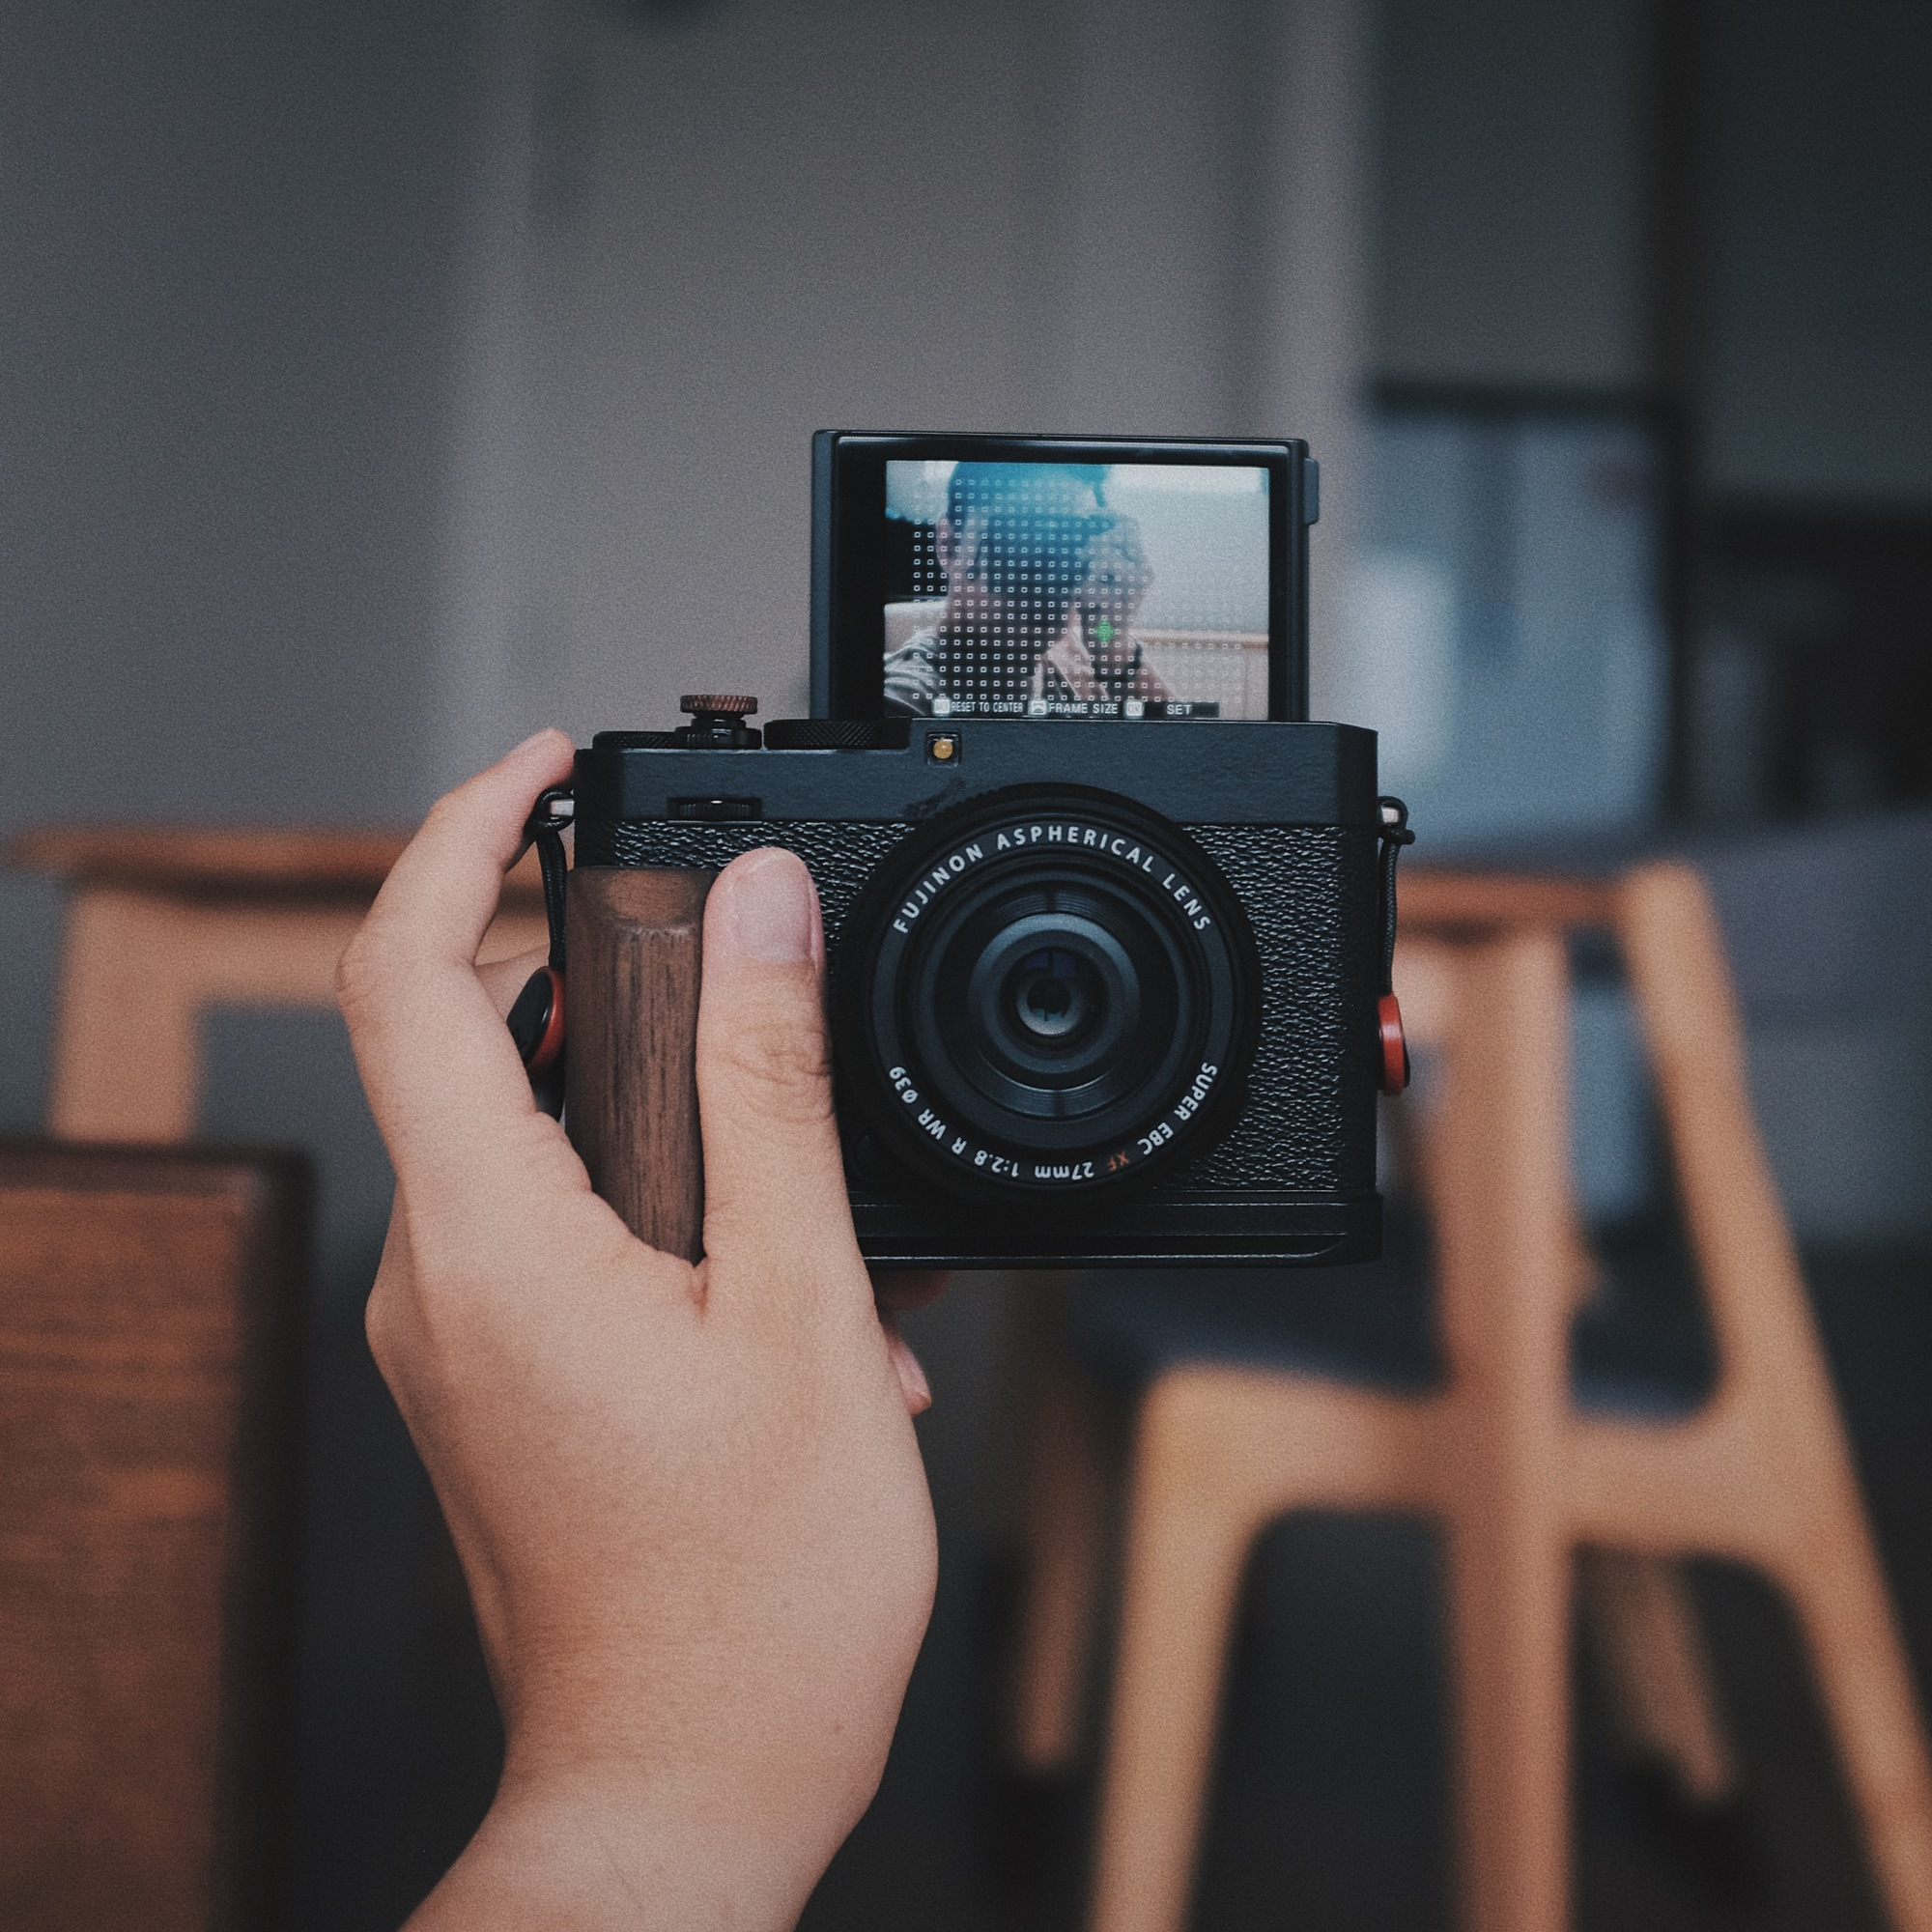
\includegraphics[width=\linewidth]{\envfinaldir/coverpic-prod.jpg}\par
            % \vskip 30pt
            \vfill

            \normalsize\rmfamily\scshape
            \copyright{} The Web Digest Project \hfill\large \envdatestr
        \end{center}
    \end{titlepage}
    % \restoregeometry
}
\newcommand{\simplehref}[1]{%
    \textcolor{blue!80!green}{\href{#1}{#1}}%
}
\renewcommand{\contentsname}{\center\Huge\sffamily\bfseries Contents\par\vskip 20pt}
\newcounter{ipartcounter}
\setcounter{ipartcounter}{0}
\newcommand{\ipart}[1]{
    % \vskip 20pt
    \clearpage
    \stepcounter{ipartcounter}
    \phantomsection
    \addcontentsline{toc}{chapter}{#1}
    % \begin{center}
    %     \Huge
    %     \sffamily\bfseries
    %     #1
    % \end{center}
    % \vskip 20pt plus 7pt
}
\newcounter{ichaptercounter}
\setcounter{ichaptercounter}{0}
\newcommand{\ichapter}[1]{
    % \vskip 20pt
    \clearpage
    \stepcounter{ichaptercounter}
    \phantomsection
    \addcontentsline{toc}{section}{\numberline{\arabic{ichaptercounter}}#1}
    \begin{center}
        \Huge
        \sffamily\bfseries
        #1
    \end{center}
    \vskip 20pt plus 7pt
}
\newcommand{\entrytitlefont}[1]{\subsection*{\raggedright\Large\sffamily\bfseries#1}}
\newcommand{\entryitemGeneric}[2]{
    % argv: title, url
    \parbox{\linewidth}{
        \entrytitlefont{#1}\par\vskip 5pt
        \footnotesize\ttfamily\mdseries
        \simplehref{#2}
    }\vskip 11pt plus 11pt minus 1pt
}
\newcommand{\entryitemGithub}[3]{
    % argv: title, url, desc
    \parbox{\linewidth}{
        \entrytitlefont{#1}\par\vskip 5pt
        \footnotesize\ttfamily\mdseries
        \simplehref{#2}\par\vskip 5pt
        \small\rmfamily\mdseries#3
    }\vskip 11pt plus 11pt minus 1pt
}
\newcommand{\entryitemAp}[3]{
    % argv: title, url, desc
    \parbox{\linewidth}{
        \entrytitlefont{#1}\par\vskip 5pt
        \footnotesize\ttfamily\mdseries
        \simplehref{#2}\par\vskip 5pt
        \small\rmfamily\mdseries#3
    }\vskip 11pt plus 11pt minus 1pt
}
\newcommand{\entryitemHackernews}[3]{
    % argv: title, hnurl, rawurl
    % \parbox{\linewidth}{
    %     \entrytitlefont{#1}\par\vskip 5pt
    %     \footnotesize\ttfamily\mdseries
    %     \simplehref{#3}\par
    %     \textcolor{black!50}{\href{#2}{#2}}
    % }\vskip 11pt plus 11pt minus 1pt
    \begin{minipage}{\linewidth}
            \entrytitlefont{#1}\par\vskip 5pt
            \footnotesize\ttfamily\mdseries
            \simplehref{#3}\par
            \textcolor{black!50}{\href{#2}{#2}}
    \end{minipage}\par\vskip 11pt plus 11pt minus 1pt
}







\begin{document}

\makeheader

\tableofcontents\clearpage




\ipart{Developers}
\ichapter{Hacker News}
\entryitemTwoLinks{U.S. stock futures tumble indicating another plummet on Wall Street}{https://news.ycombinator.com/item?id=43605670}{https://www.reuters.com/markets/us/us-investors-braced-more-volatility-bumps-ahead-monday-trading-open-2025-04-06/}

\entryitemTwoLinks{Rsync replaced with openrsync on macOS Sequoia}{https://news.ycombinator.com/item?id=43605003}{https://derflounder.wordpress.com/2025/04/06/rsync-replaced-with-openrsync-on-macos-sequoia/}

\entryitemTwoLinks{Gmail E2E is as terrible as expected}{https://news.ycombinator.com/item?id=43604308}{https://michal.sapka.pl/2025/gmail-e2e-is-as-terrible-as-expected/}

\entryitemTwoLinks{Gumroad's Interestingly Timed "Open-Source" Play}{https://news.ycombinator.com/item?id=43603999}{https://tedium.co/2025/04/06/gumroad-open-source-doge-drama/}

\entryitemTwoLinks{Recent AI model progress feels mostly like bullshit}{https://news.ycombinator.com/item?id=43603453}{https://www.lesswrong.com/posts/4mvphwx5pdsZLMmpY/recent-ai-model-progress-feels-mostly-like-bullshit}

\entryitemTwoLinks{E.U. Prepares Major Penalties Against X}{https://news.ycombinator.com/item?id=43603307}{https://www.nytimes.com/2025/04/03/technology/eu-penalties-x-elon-musk.html}

\entryitemTwoLinks{Federal cuts disrupt repairs to iconic U.S. trails}{https://news.ycombinator.com/item?id=43603111}{https://apnews.com/article/pacific-crest-appalachian-trail-federal-layoffs-934a5526570569b625f5d854ec339a04}

\entryitemTwoLinks{Max severity RCE flaw discovered in widely used Apache Parquet}{https://news.ycombinator.com/item?id=43603091}{https://www.bleepingcomputer.com/news/security/max-severity-rce-flaw-discovered-in-widely-used-apache-parquet/}

\entryitemTwoLinks{Peter Navarro Invented an Expert for His Books, Based on Himself (2019)}{https://news.ycombinator.com/item?id=43602777}{https://www.nytimes.com/2019/10/16/us/politics/peter-navarro-ron-vara.html}

\entryitemTwoLinks{Self-Driving Teslas Are Fatally Rear-Ending Motorcyclists More Than Any Other}{https://news.ycombinator.com/item?id=43601421}{https://fuelarc.com/news-and-features/self-driving-teslas-are-fatally-striking-motorcyclists-more-than-any-other-brand-new-analysis/}

\entryitemTwoLinks{How the Atlantic's Jeffrey Goldberg Got Added to the White House Signal Chat}{https://news.ycombinator.com/item?id=43601213}{https://www.theguardian.com/us-news/2025/apr/06/signal-group-chat-leak-how-it-happened}

\entryitemTwoLinks{Neutron Stars Hint at Another Dimension}{https://news.ycombinator.com/item?id=43600704}{https://nautil.us/neutron-stars-hint-at-another-dimension-1202180/}

\entryitemTwoLinks{The ``S'' in MCP Stands for Security}{https://news.ycombinator.com/item?id=43600192}{https://elenacross7.medium.com/\%EF\%B8\%8F-the-s-in-mcp-stands-for-security-91407b33ed6b}

\entryitemTwoLinks{SeedLM: Compressing LLM Weights into Seeds of Pseudo-Random Generators}{https://news.ycombinator.com/item?id=43599967}{https://machinelearning.apple.com/research/seedlm-compressing}

\entryitemTwoLinks{Video footage appears to contradict Israeli account of Gaza medic killings}{https://news.ycombinator.com/item?id=43599864}{https://www.bbc.com/news/articles/c4g2z103nqxo}

\entryitemTwoLinks{Standard Ebooks: liberated ebooks, carefully produced for the true book lover}{https://news.ycombinator.com/item?id=43599637}{https://standardebooks.org}

\entryitemTwoLinks{My Browser WASM't Prepared for This. Using DuckDB, Apache Arrow and Web Workers}{https://news.ycombinator.com/item?id=43599613}{https://motifanalytics.medium.com/my-browser-wasmt-prepared-for-this-using-duckdb-apache-arrow-and-web-workers-in-real-life-e3dd4695623d}

\entryitemTwoLinks{Apple's Darwin OS and XNU Kernel Deep Dive}{https://news.ycombinator.com/item?id=43597778}{https://tansanrao.com/blog/2025/04/xnu-kernel-and-darwin-evolution-and-architecture/}

\entryitemTwoLinks{The ADHD body double: A unique tool for getting things done}{https://news.ycombinator.com/item?id=43597425}{https://add.org/the-body-double/}

\entryitemTwoLinks{Rules for Negotiating a Job Offer (2016)}{https://news.ycombinator.com/item?id=43596864}{https://haseebq.com/my-ten-rules-for-negotiating-a-job-offer/}\ichapter{Phoronix}
\entryitemGeneric{\hskip 0pt{}Linux 6.15-rc1 Released With New Performance Optimizations, Updated Zstd \& New Hardware}{https://www.phoronix.com/news/Linux-6.15-rc1-Released}

\entryitemGeneric{\hskip 0pt{}NVIDIA Makes PhysX \& Flow GPU Code Open-Source}{https://www.phoronix.com/news/NVIDIA-OSS-PhysX-Flow-GPU}

\entryitemGeneric{\hskip 0pt{}Apple Z2 Touchscreen / Touch Bar Driver Lands In Linux 6.15}{https://www.phoronix.com/news/Linux-6.15-Input}

\entryitemGeneric{\hskip 0pt{}PostgreSQL Turns To AVX-512 For CRC32 Computations: Up To 3x Faster}{https://www.phoronix.com/news/PostgreSQL-CRC32C-AVX512}

\entryitemGeneric{\hskip 0pt{}Large Atomic Write Preparations Land In Linux 6.15}{https://www.phoronix.com/news/Linux-Preps-Large-Atomic-Write}

\entryitemGeneric{\hskip 0pt{}Linux 6.15 Performance Events Adds Support For AMD Zen 5 Load Latency Filtering}{https://www.phoronix.com/news/Linux-6.15-Perf-Events}

\entryitemGeneric{\hskip 0pt{}Linux 6.15 Kbuild Adds Support For LoongArch Debian \& Faster gendwarfksyms}{https://www.phoronix.com/news/Linux-6.15-Kbuild}

\entryitemGeneric{\hskip 0pt{}Linux 6.15 Crypto Subsystem Delivers Faster AES-CTR For AMD Zen 5 \& Other x86\_64 CPUs}{https://www.phoronix.com/news/Linux-6.15-Crypto}

\entryitemGeneric{\hskip 0pt{}RISC-V With Linux 6.15 Adds Support For BFloat16 "BF16" Instructions}{https://www.phoronix.com/news/Linux-6.15-RISC-V}\ichapter{Dribbble}
\entryitemGeneric{\hskip 0pt{}Educational Website on Space Pollution}{https://dribbble.com/shots/25860515-Educational-Website-on-Space-Pollution}

\entryitemGeneric{\hskip 0pt{}CRYSTAL PRT\_2 // Mobile Version}{https://dribbble.com/shots/25860264-CRYSTAL-PRT-2-Mobile-Version}

\entryitemGeneric{\hskip 0pt{}LA Kings Mexican Heritage Theme Night Art}{https://dribbble.com/shots/25862720-LA-Kings-Mexican-Heritage-Theme-Night-Art}

\entryitemGeneric{\hskip 0pt{}Going for Gold}{https://dribbble.com/shots/25861716-Going-for-Gold}

\entryitemGeneric{\hskip 0pt{}Atomiq Unused Logo Design}{https://dribbble.com/shots/25861903-Atomiq-Unused-Logo-Design}

\entryitemGeneric{\hskip 0pt{}Ship Logo Design - Boat, Shield, Star, Waves}{https://dribbble.com/shots/25854151-Ship-Logo-Design-Boat-Shield-Star-Waves}

\entryitemGeneric{\hskip 0pt{}Investment fund bank hero shot}{https://dribbble.com/shots/25855871-Investment-fund-bank-hero-shot}

\entryitemGeneric{\hskip 0pt{}Interactive Speed Slider}{https://dribbble.com/shots/25851176-Interactive-Speed-Slider}

\entryitemGeneric{\hskip 0pt{}Abstract}{https://dribbble.com/shots/25853030-Abstract}

\entryitemGeneric{\hskip 0pt{}Croc logo}{https://dribbble.com/shots/25852607-Croc-logo}

\entryitemGeneric{\hskip 0pt{}Jot Landing Page, Website Design, business web site}{https://dribbble.com/shots/25843658-Jot-Landing-Page-Website-Design-business-web-site}

\entryitemGeneric{\hskip 0pt{}Logo Design Selection Q1 2025}{https://dribbble.com/shots/25852275-Logo-Design-Selection-Q1-2025}

\entryitemGeneric{\hskip 0pt{}Cloud Lightning}{https://dribbble.com/shots/25852815-Cloud-Lightning}

\entryitemGeneric{\hskip 0pt{}ef monogram}{https://dribbble.com/shots/25847206-ef-monogram}

\entryitemGeneric{\hskip 0pt{}Helpfull - Logo Redesign}{https://dribbble.com/shots/25847828-Helpfull-Logo-Redesign}

\entryitemGeneric{\hskip 0pt{}Outrigger Marketing Logo}{https://dribbble.com/shots/25848681-Outrigger-Marketing-Logo}

\entryitemGeneric{\hskip 0pt{}Wayflow Logo Design - Letter W, Waves, Flow}{https://dribbble.com/shots/25847473-Wayflow-Logo-Design-Letter-W-Waves-Flow}

\entryitemGeneric{\hskip 0pt{}Prana Symbol}{https://dribbble.com/shots/25847656-Prana-Symbol}

\entryitemGeneric{\hskip 0pt{}Letter G set}{https://dribbble.com/shots/25845864-Letter-G-set}

\entryitemGeneric{\hskip 0pt{}Let down your hair}{https://dribbble.com/shots/25844844-Let-down-your-hair}

\entryitemGeneric{\hskip 0pt{}Chat GPT 4 Branding Concept}{https://dribbble.com/shots/25844194-Chat-GPT-4-Branding-Concept}

\entryitemGeneric{\hskip 0pt{}Sustainable contribution selector: percentage picker}{https://dribbble.com/shots/25843734-Sustainable-contribution-selector-percentage-picker}

\entryitemGeneric{\hskip 0pt{}FG}{https://dribbble.com/shots/25842733-FG}

\entryitemGeneric{\hskip 0pt{}Kovre Winery Logo Exploration}{https://dribbble.com/shots/25844706-Kovre-Winery-Logo-Exploration}


\ipart{Developers~~~~(zh-Hans)}
\ichapter{Solidot}
\entryitemGeneric{\hskip 0pt{} 《星际公民(Star Citizen)》筹款突破八亿美元}{https://www.solidot.org/story?sid=80976}

\entryitemGeneric{\hskip 0pt{}一名微软雇员干扰了公司五十周年庆}{https://www.solidot.org/story?sid=80975}

\entryitemGeneric{\hskip 0pt{}特朗普再给予 TikTok 75 天宽限期}{https://www.solidot.org/story?sid=80974}

\entryitemGeneric{\hskip 0pt{}天文学家在附近发现将碰撞的双星系统}{https://www.solidot.org/story?sid=80973}

\entryitemGeneric{\hskip 0pt{}细菌氧代谢出现时间早于地球大氧化事件 }{https://www.solidot.org/story?sid=80972}

\entryitemGeneric{\hskip 0pt{}空调驱动全球能源需求增长}{https://www.solidot.org/story?sid=80971}

\entryitemGeneric{\hskip 0pt{}倭黑猩猩声音具有与人类语言相似的组合性}{https://www.solidot.org/story?sid=80970}

\entryitemGeneric{\hskip 0pt{}为何 AV1 仍未普及?}{https://www.solidot.org/story?sid=80969}

\entryitemGeneric{\hskip 0pt{}英特尔和台积电达成初步协议合资运营芯片制造业务}{https://www.solidot.org/story?sid=80968}\ichapter{V2EX}
\entryitemGeneric{\hskip 0pt{}[机器学习] 什么?唠唠嗑就能生成游戏关卡! Unreal Engine + MCP 来了!}{https://www.v2ex.com/t/1123593}

\entryitemGeneric{\hskip 0pt{}[投资] 相信国运,定投纳指的人有福了}{https://www.v2ex.com/t/1123592}

\entryitemGeneric{\hskip 0pt{}[哔哩哔哩] 吐槽一下 B 站网页主页推荐}{https://www.v2ex.com/t/1123590}

\entryitemGeneric{\hskip 0pt{}[问与答] 明天很可能会股灾,有仓位的,睡得着吗?}{https://www.v2ex.com/t/1123589}

\entryitemGeneric{\hskip 0pt{}[问与答] 给老人选配安卓平板, vivo 还是红米?}{https://www.v2ex.com/t/1123588}

\entryitemGeneric{\hskip 0pt{}[问与答] 家用服务器有推荐的吗?}{https://www.v2ex.com/t/1123587}

\entryitemGeneric{\hskip 0pt{}[分享发现] Folo (Follow) 中文界面来了}{https://www.v2ex.com/t/1123586}

\entryitemGeneric{\hskip 0pt{}[职场话题] 来日本五年,一直干派遣,今年刚上岸日本公司自社开发正社员。}{https://www.v2ex.com/t/1123585}

\entryitemGeneric{\hskip 0pt{}[分享创造] 基于 mermaid 实现了一个 uml 的画图工具}{https://www.v2ex.com/t/1123584}

\entryitemGeneric{\hskip 0pt{}[分享创造] 用 cursor 肝了 3 个月,搞了个聚合搜索的浏览器扩展,有喜欢的吗}{https://www.v2ex.com/t/1123583}

\entryitemGeneric{\hskip 0pt{}[酷工作] [北京/上海/杭州/深圳] 抖音-基础技术-同学,你喜欢 Swift 吗?}{https://www.v2ex.com/t/1123582}

\entryitemGeneric{\hskip 0pt{}[旅行] 五一旅游,租 s23u/s24u 而不是相机拍照可行吗?}{https://www.v2ex.com/t/1123580}

\entryitemGeneric{\hskip 0pt{}[Intel] 解决 intel N510x cpu 虚拟化下网口断流 Bug}{https://www.v2ex.com/t/1123579}

\entryitemGeneric{\hskip 0pt{}[问与答] 要到微信后怎么发展感情}{https://www.v2ex.com/t/1123578}

\entryitemGeneric{\hskip 0pt{}[程序员] 微信 4.0 桌面端生成新的文件夹位置,导致以前的资料没同步}{https://www.v2ex.com/t/1123577}

\entryitemGeneric{\hskip 0pt{}[宽带症候群] 有没有北京移动宽带的上行速率被限制的? PT 用户}{https://www.v2ex.com/t/1123575}

\entryitemGeneric{\hskip 0pt{}[Python] 我参考 VSCode 设计了一个多层级配置框架,专为框架开发者设计}{https://www.v2ex.com/t/1123573}

\entryitemGeneric{\hskip 0pt{}[问与答] 有不冲会员能听大部分互联网歌曲的 APP 或者平台吗。}{https://www.v2ex.com/t/1123572}

\entryitemGeneric{\hskip 0pt{}[NAS] 致态 SE005 SATA SSD 怎么样?}{https://www.v2ex.com/t/1123571}

\entryitemGeneric{\hskip 0pt{}[生活] 怎么看病才能不被宰}{https://www.v2ex.com/t/1123570}

\entryitemGeneric{\hskip 0pt{}[问与答] win10 任务栏 刚开机后 不显示打开的软件,但过一会就正常?}{https://www.v2ex.com/t/1123567}

\entryitemGeneric{\hskip 0pt{}[GitHub Copilot] GitHub Copilot 正式开放 MCP 预览了}{https://www.v2ex.com/t/1123566}

\entryitemGeneric{\hskip 0pt{}[教育] 高考专项计划志愿填报}{https://www.v2ex.com/t/1123565}

\entryitemGeneric{\hskip 0pt{}[问与答] 清华大学的非全 MEM 值得读么?}{https://www.v2ex.com/t/1123564}

\entryitemGeneric{\hskip 0pt{}[Android] 刚看了钟文泽 OPPO Find X8s 的评测视频,这 AI 功能集成得太好了,走🍎的路让🍎无路可走 🤣}{https://www.v2ex.com/t/1123563}

\entryitemGeneric{\hskip 0pt{}[程序员] 在 AI 的辅助下,独立开发了一个拼图游戏(jigsaw puzzle)}{https://www.v2ex.com/t/1123562}

\entryitemGeneric{\hskip 0pt{}[Telegram] 各位 v 友有没有常用的 telegram stickers 推荐,最好就是贱兮兮的}{https://www.v2ex.com/t/1123561}

\entryitemGeneric{\hskip 0pt{}[问与答] 京东自营还靠谱吗}{https://www.v2ex.com/t/1123560}

\entryitemGeneric{\hskip 0pt{}[分享创造] web 缓存网上线网站 logo 加速服务啦!可申请加入您的 logo}{https://www.v2ex.com/t/1123559}

\entryitemGeneric{\hskip 0pt{}[Windows] DDR5 128GB 内存 Windows 11 一周不关机必蓝屏 是系统问题还是 DDR5 的问题?每次报错都不一样,各种错误都有}{https://www.v2ex.com/t/1123558}

\entryitemGeneric{\hskip 0pt{}[分享创造] X86-64 位简易系统开发 - 从 BIOS 阶段开始}{https://www.v2ex.com/t/1123557}

\entryitemGeneric{\hskip 0pt{}[分享创造] 我用 leafletjs 做了一个世界地铁地图网站,大家看看}{https://www.v2ex.com/t/1123556}

\entryitemGeneric{\hskip 0pt{}[路由器] 大唐 EHL35-J6412 说明书 V0.5(MC200) 单板计算机 适合做软路由 3.5 寸}{https://www.v2ex.com/t/1123555}

\entryitemGeneric{\hskip 0pt{}[生活] [hair selfie]-2025-04-06}{https://www.v2ex.com/t/1123554}

\entryitemGeneric{\hskip 0pt{}[分享创造] [开源] EvanNav:一个审美在线儿的 HR 用 AI 写的手机/PC 网络收藏夹}{https://www.v2ex.com/t/1123551}

\entryitemGeneric{\hskip 0pt{}[VXNA] 个人博客申请收款—pipuwong.com}{https://www.v2ex.com/t/1123549}

\entryitemGeneric{\hskip 0pt{}[YouTube] youtube 安卓小米手机,播放大概半分钟到一分钟就会卡住,怎么解决?}{https://www.v2ex.com/t/1123548}

\entryitemGeneric{\hskip 0pt{}[PHP] 推荐个好用的集成环境}{https://www.v2ex.com/t/1123546}

\entryitemGeneric{\hskip 0pt{}[MacBook Air] mba m1 丐版内存空间不够了,有什么好的解决办法吗}{https://www.v2ex.com/t/1123545}

\entryitemGeneric{\hskip 0pt{}[音乐] [30 岁学电吉他入门分享] 装备 2500 块左右 + 免费的 B 站练习教程}{https://www.v2ex.com/t/1123544}

\entryitemGeneric{\hskip 0pt{}[程序员] 对于一个语言新手来说, AI 辅助生成的代码片段是不是能称得上``质量较高''的代码学习指导}{https://www.v2ex.com/t/1123543}

\entryitemGeneric{\hskip 0pt{}[V2EX] v2ex 考虑推出一个 mcp server 吗?}{https://www.v2ex.com/t/1123540}

\entryitemGeneric{\hskip 0pt{}[OpenAI] 关于 ChatGPT 的回答好像要越来越非 ai 化了?一下子甚至觉得有点点人样了?}{https://www.v2ex.com/t/1123539}

\entryitemGeneric{\hskip 0pt{}[职场话题] Gap 半年,三十岁程序员找工作记录 day14}{https://www.v2ex.com/t/1123538}

\entryitemGeneric{\hskip 0pt{}[React] react native 有类似 antd/x 的 ai 对话组件库吗}{https://www.v2ex.com/t/1123537}

\entryitemGeneric{\hskip 0pt{}[求职] 成都 7 年 Java /3 年 GO 等个机会~}{https://www.v2ex.com/t/1123536}

\entryitemGeneric{\hskip 0pt{}[智能家电] 小米智能开关值得入手吗}{https://www.v2ex.com/t/1123535}

\entryitemGeneric{\hskip 0pt{}[游戏] 企鹅冲刺小游戏~~}{https://www.v2ex.com/t/1123534}

\entryitemGeneric{\hskip 0pt{}[macOS] 再自荐下自写的一个 Finder 的 Quick Action - Image Kit App 送兑换码}{https://www.v2ex.com/t/1123533}

\entryitemGeneric{\hskip 0pt{}[Terminal] Kitty, Wezterm, Alacritty, Ghostty 该用哪个?}{https://www.v2ex.com/t/1123532}


\ipart{Generic News}







\clearpage
\leavevmode\vfill
\footnotesize

Copyright \copyright{} 2023-2025 Neruthes and other contributors.

This document is published with CC BY-NC-ND 4.0 license.

The entries listed in this newsletter may be copyrighted by their respective creators.

This newsletter is generated by the Web Digest project.

The newsletters are also delivered via Telegram channel \CJKunderline{\href{https://t.me/webdigestchannel}{https://t.me/webdigestchannel}}.\\
RSS feed is available at \CJKunderline{\href{https://webdigest.pages.dev/rss.xml}{https://webdigest.pages.dev/rss.xml}}.

This newsletter is available in PDF at
\CJKunderline{\href{https://webdigest.pages.dev/}{https://webdigest.pages.dev/}}.

The source code being used to generate this newsletter is available at\\
\CJKunderline{\href{https://github.com/neruthes/webdigest}{https://github.com/neruthes/webdigest}}.

This newsletter is also available in
\CJKunderline{\href{http://webdigest.pages.dev/readhtml/\envyear/WebDigest-20250407.html}{HTML}} and
\CJKunderline{\href{https://github.com/neruthes/webdigest/blob/master/markdown/\envyear/WebDigest-20250407.md}{Markdown}}.


\coverpic{https://unsplash.com/photos/orange-sunset-over-dark-mountains-and-clouds-d-vYj8A-JQ8}{Claudio Schwarz}


\end{document}
